\documentclass[conference]{IEEEtran}
\IEEEoverridecommandlockouts
\usepackage{graphicx}
\usepackage{algorithm}
\usepackage{algorithmicx}
\usepackage{algpseudocode}
\usepackage[dvipsnames]{xcolor}
\usepackage{amsmath}
\usepackage{hyperref}
\usepackage{caption}
\usepackage{subcaption}

\algblock{Input}{EndInput}
\algnotext{EndInput}
\algblock{Output}{EndOutput}
\algnotext{EndOutput}
\newcommand{\Desc}[2]{\State \makebox[2em][l]{#1}#2}

\newcommand{\tristan}[1]{\color{orange}\textbf{From Tristan:}#1\color{black}}
\newcommand{\valerie}[1]{\color{blue}\textbf{From Valerie:}#1\color{black}}


\begin{document}
\title{I/O simulation model with Linux page cache, integration and evaluation in SimGrid framework}

\author{\IEEEauthorblockN{Hoang-Dung Do, Val\'erie Hayot-Sasson, Rafael Ferreira da Silva, Henri Casanova, Tristan Glatard
  }\\
  \IEEEauthorblockA{
    Department of Computer Science and Software Engineering, Concordia University, Montreal, Canada
  }
}

\maketitle

	\begin{abstract}
		\begin{itemize}
			\item The I/O bottleneck in HPC and the need of experiments.
			\item HPC experiment frameworks and advantages of SimGrid.
			\item The missing of the ability to simulate page cache, the goal of this paper.
			\item Principle of the simulator, experiment scenarios and comparisons.
			\item Brief discussion on results and future work.
		\end{itemize}
	\end{abstract}

	\section{Introduction}
		\begin{itemize}
			\item HPC, the bottleneck in I/O and the demand of HPC experiments. 
			\item Difficulties in conducting high performance computing experiments and the need of simulation frameworks.
			\item Existing experiment methods, simulators, simulation frameworks. The advantages of SimGrid compared to others \cite{simgrid2008, lebre2015}. The missing of the ability to simulate page cache in SimGrid \cite{lebre2015}.
			\item The objective of the paper: Add capability to simulate I/O with page cache in SimGrid.
			\item Clarify, distinguish between memory I/O (i/o to page cache) and disk I/O.
		\end{itemize}
	\section{Related Work}			
		
		\subsection{Page cache}
			\begin{itemize}
				\item What is page cache? How it works \cite{linuxdev3rd2010}. 
				Write-back vs writethrough and direct i/o. Effects and importance of page cache.
				\item Introduce some existing strategies with some highlighted pros and cons.
				\item Current implementation in Linux and some reasons why it is chosen to be implemented (implementation complexity, effectiveness, overhead, etc) \cite{linuxdev3rd2010}
				\item \tristan{LRU lists are mentioned in the next section, they should be described here.}
			\end{itemize}									

		\subsection{Simulators}
			\begin{itemize}
				\item Discuss some existing methods, simulation frameworks to conduct HPC experiments. Compare pros and cons (accuracy, simulation time, usability) of some simulators (SimGrid, GridSim).
				\item Related development: RAM energy consumption \cite{gill2019} \cite{ouarnoughi2017} 
				\item What is implemented in simulators that useful for our model:
				distinguished and shared bandwidths, concurrency, device latency. 
				\item Discuss the pros of SimGrid and the reasons why we chose it to conduct experiments. (Section 2.2.2 in \cite{simgrid2014})
				\item Introduce WRENCH and it's advantage.
				\item \tristan{Mention the status of storage simulation in simulators, so that we understand from Fig 1 that storage devices are available}
			\end{itemize}
			
	\section{Method}

		In this section, we present our approach to model file read and write with
		I/O to page cache, cache eviction and data flushing mechanisms implemented 
		in the Linux kernel. We also detail the design of our simulators and their
		implementation. Finally, we describe experimental scenarios to evaluate
		our simulation model on real applications using a standalone Python
		prototype, SimGrid framework using original WRENCH and the WRENCH version 
		that is integrated with our simulation model (WRENCH-Ext).

		\subsection{Principle of the simulator}
	
            We separate our simulation model in two components, the IO
			Controller and the Memory Manager, which together simulate 
			file read/write mechanisms in Linux (Figure~\ref{fig:interaction}). 
			The Memory Manager simulates I/Os to cache, flushing, periodical flushing, 
			and cache eviction, whereas the IO Controller simulates file reads and writes. 
			Simulated applications can simply interact with the IO Controller instead of 
			calling simulated storage directly as is the case with current simulators.

			\begin{figure}
   				\centering
   				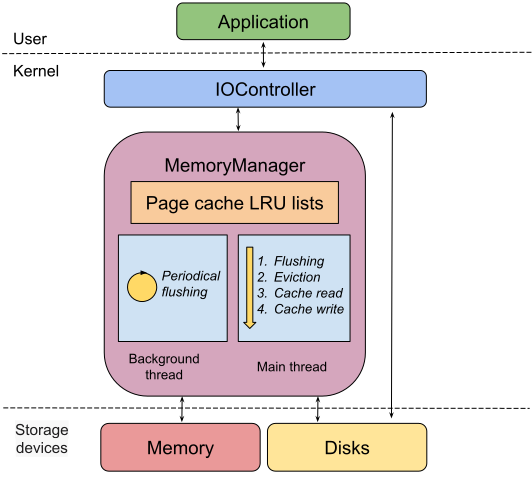
\includegraphics[width=0.85\columnwidth]{figures/interaction.pdf}
   				\caption{Overview of the simulated write-back page cache}\label{fig:interaction}
			\end{figure}	

			\subsubsection{Memory simulation model}
			
			We leverage existing storage simulation models to simulate the memory,
			which is characterized with storage capacity, distinguished read/write 
			bandwidths and device latency. 
			All of these features are dealt within models in simulation 
			frameworks, which makes storage models applicable to memory \cite{lebre2015}. 
			In addition, leveraging existing disk models allows us 
			to take advantage of bandwidth sharing between concurrent disk I/O to 
			simulate parallel memory accesses.\tristan{we should refer to related work, 
            see comment there} \valerie{Agreed. It's unclear how existing storage models enable this at the moment}.

			Memory Manager simulates two parallel threads. The first thread is the 
			main thread where activities of applications are simulated, and responsible 
			for the simulation of data flushing, cache eviction and I/Os to cache. 
			The second thread is a simulated background thread, in which Memory Manager 
			periodically searches and flushes expired dirty data in page cache LRU lists 
			to disks. 

			In Linux kernel, the page cache LRU lists contain file pages. However, 
			due to the large number of file pages, managing lists of pages may 
			require significant computation overhead. 
			Thus, we introduce the concept of a data block as a unit to represent data 
			cached in memory. A data block is a subset of file pages stored in
            page cache that were accessed in the same I/O operation. 
			A data block has information about file name, block size, last access 
			time, a dirty flag that represents whether the data is clean (0) 
			or dirty (1), and the time it is written to cache as dirty data. 
			Blocks can have different sizes and a given file can have multiple 
			data blocks in page cache. In addition, a data block can be split into an 
			arbitrary number of smaller blocks.

			\begin{figure}
   				\centering
   				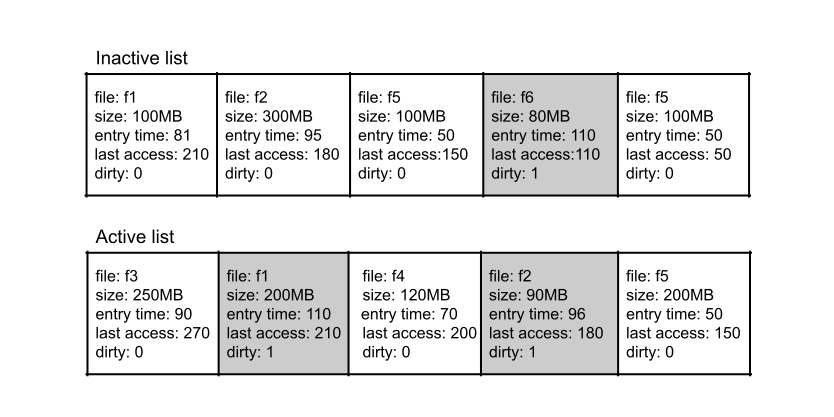
\includegraphics[width=\columnwidth]{figures/lru_lists.pdf}
   				\caption{Simulation of page cache LRU lists with data blocks}	\label{fig:lrulist}
			\end{figure}	
			
			Now, page cache LRU lists can be modeled with two lists of data blocks: 
			an active list and an inactive list, ordered by last access time 
			(earliest first, see Figure~\ref{fig:lrulist}).
			As in the kernel, our simulator keeps the size of the active list under
			twice the size of the inactive list by moving least recently 
            used data blocks from the active list to the inactive list.
			Modeling page cache LRU lists as lists of data blocks reduces the
			overhead of the simulator, as data blocks are obviously less
			numerous than file pages, while achieving the accuracy in I/O time
			simulation that can be seen in the later section.
			
			Given an arbitrary file, at a specific time, it can be partially cached, 
			completely cached, or uncached.
			Cached data is composed of data blocks existing in either or both
            of the page cache LRU lists. Cached blocks reside in the inactive list
            unless they have been recently reaccessed. Cached blocks 
            located on the inactive list that are subsequently accessed, 
            will be moved to the top of the active list. Cached blocks 
            recently written to cache are dirty blocks until they are flushed to disk.

            Our model supports chunk-by-chunk file read/write simulation
            with an user-defined chunk size, in which chunks are read/written 
            until file is entirely read/written. 
            The simulated LRU lists are used as follows. 
            When a file is read, its data can be partially cached, completely cached, 
            or uncached. 
            Uncached data is read from disk first, and cached data is only read 
            after all uncached data is read (left to right in Figure~\ref{fig:read_order}).
            When a chunk of uncached data is read, a new clean block is created 
            and put to the top of the inactive list. 
            For a chunk of cached data, because one or more existing data blocks 
            in two page cache LRU lists are accessed again, read dirty blocks are 
            moved to the active list, while clean data blocks are merged into 
            a single clean block and then also put in the active list. 
			The reason we do not merge dirty blocks is that different blocks 
			are written to cache at different time, and this time is used later for 
			periodical flushing process.
			In case a block is not entirely read, it is split into two smaller blocks, 
			one is reaccessed and the other remains the same.
			
			\begin{figure}
   				\centering
   				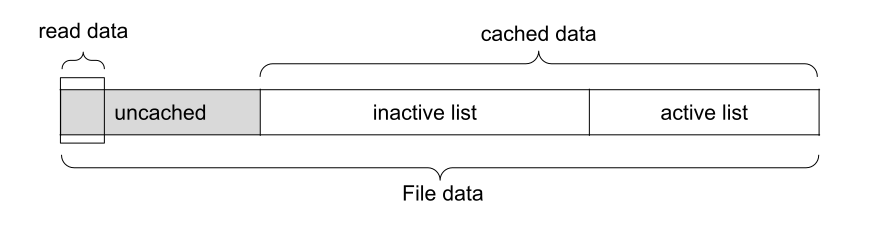
\includegraphics[width=\columnwidth]{figures/read_order.pdf}
   				\caption{File data read order}	\label{fig:read_order}
			\end{figure}	
			
			In the case of writing data, we can assume that all data to be written is 
			uncached and it is written to cache as dirty data. 
			Thus, each time a chunk is written, we create a block of dirty data and 
			put it in the inactive list.
			
			\textcolor{red}{[Is there any kind of accesses other than read and write?]}. 			
			
            As is done in the kernel, we ensure the size of the active list does not 
            exceed twice the size of the inactive list 
			\cite{gorman2004understanding, linuxdev3rd2010}. 
			This is done by moving least recently used blocks in the active list 
			to the inactive list when the active list grows. If only a part of a data 
			block needs to be moved, the block is split.

			Next, we simulate data flushing, which runs on the main simulated 
			thread and writes back dirty data to disk. 
			The data flushing simulation function traverses the sorted 
			inactive list first, and then the active list, looks for least recently used 
			dirty blocks, writes them to disk through the storage device model, 
			and sets dirty flags of these blocks to 0 until the total flushed amount 
			reaches the amount to be flushed or there is no dirty data left in cache. 
			If the last flushed block is not entirely flushed, it is split into 
			two blocks, one that is flushed and one that remains dirty.
			The flushing time is simulated with storage model.
				
			Similarly to data flushing, our cache eviction simulation runs on 
			the main thread, frees up the page cache by traversing and deleting 
			least recently used clean data blocks in the inactive list.
			The amount of evicted data is passed in and data blocks are deleted 
			from the inactive list until total evicted data reaches the amount 
			passed in, or there is no clean block left in the list.
			If the last evicted block is not entirely evicted, the block is split, 
			and only one block is deleted.
			The cache eviction simulation does not add up to the simulated time 
			since cache eviction time is negligible in real systems.		
			
			\begin{algorithm}\caption{Periodical flushing simulation}\label{alg:pdflush}
				\small
				\begin{algorithmic}[1]
					\Input
        				\Desc{in}{page cache inactive list}
        				\Desc{ac}{page cache active list}
						\Desc{t}{predefined flushing time interval}
						\Desc{sm}{storage simulation model}
   					\EndInput
   					\While{host is on}
						\State blocks = expired dirty blocks in active and inactive list
						\State flushing\_time = sm.write(blocks)
						\State Flag blocks as clean data
						\If{flushing\_time $<$ t}
							\State sleep(t - flushing\_time)
						\EndIf
					\EndWhile
				\end{algorithmic}
			\end{algorithm}				
			
			The periodical flushing simulation is run on a simulated background thread 
			to flush expired dirty data blocks from cache to disk.
			Similar to expired dirty pages in real Linux systems, a dirty block in our model 
			is considered expired if the time it remains in cache as dirty is longer than 
			the predefined expire time. This time is counted from the time it is written 
			to cache to current simulated time. 
			The simulation algorithm of periodical flushing is an infinite loop in which 
			Memory Manager searches and flushes these expired dirty blocks to disk, 
			as described in Algorithm~\ref{alg:pdflush}. 
			The loop ends when the host the host is off (line 6). 
			In each repetition, Memory Manager finds expired dirty blocks in two 
			page cache LRU lists (line 7), simulates writes of data of these blocks 
			to disk (line 8), and mark them as clean (line 9).
			If the flushing time does not exceed our time interval, the thread is put 
			to sleep for the remaining time (lines 10-12). 
			Then based on the state of the host at current simulated time, 
			the algorithm continues or finishes the loop .
			Because periodical flushing is simulated as a background thread, it can be 
			concurrent with disk I/O on main thread. This parallelism is handled by the 
			storage model and reflected in simulated I/O time. 	

			\subsubsection{File I/O simulation model}			
			 
			When simulated applications need to read/write a file, they can simply call 
			the IO Controller instead of the storage simulation models. 
			\tristan{this should move, not sure where for now: 
			Because every computer has its own memory and system configurations, 
			one IO Controller object and one Memory Manager object are created 
			for each simulated host.}
			
			As mentioned, in our model, a file read/write can be complete by read/write 
			chunk-by-chunk until entire file is read/written.
			To read or write a chunk of file, a simulated application sends a request to the 
			IOController instance on the node where the requested file is stored.
			Based on the memory status in Memory Manager, the IOController 
			orchestrates cache and disk reads/writes, flushing, cache eviction 
			to simulate I/O time.
			
			\begin{algorithm}\caption{File chunk read simulation}\label{alg:read}
				\small
				\begin{algorithmic}[1]
					\Input
        				\Desc{cs}{chunk size}
        				\Desc{fn}{file name}
        				\Desc{fs}{file size (assume to fit in memory)}
						\Desc{mm}{MemoryManager object}
						\Desc{sm}{storage simulation model}
   					\EndInput
   					\State disk\_read = min(cs, fs - mm.cached(fn))
   					\State cache\_read = cs - disk\_read
					\State mm.flush(cs + disk\_read - mm.free\_mem - mm.evictable, fn) 
					\State mm.evict(cs + disk\_read - mm.free\_mem, fn) 
					\If {disk\_read $>$ 0}  \Comment{Read uncached data}	
						\State sm.read(disk\_read)  
						\State mm.add\_to\_cache(disk\_read, fn) 	
					\EndIf
					\If {cache\_read $>$ 0} \Comment{Read cached}
						\State mm.cache\_read(cache\_read)  
					\EndIf
				\end{algorithmic}
			\end{algorithm}			
			
			The algorithm to simulate a chunk read is described in Algorithm~\ref{alg:read}.   
			When a simulated application read a chunk of a file, it sends a 
			chunk read request to IO Controller. 
			First, we calculate the amount of uncached data that needs to be read 
			from disk, and the remaining amount is read from cache (line 7-8).
			We assume that after a file is read, there are two copies of the file in memory 
			(one in cache, one in anonymous memory). 
			Thus, when a chunk is read, one copy of the chunk occupies anonymous memory, 
			and the uncached part of that chunk is read into cache.	
			The amount of required memory to read the chunk is calculate and 
			if there is not enough memory available, Memory Manager is called to 
			flush dirty data to disk and simulate flushing time with memory model (line 9).
			This flushing is complemented by eviction in the Memory Manager (line 10). 
			Then, if there is uncached data, a disk read is simulated with disk model (line 12), 
			and this data of the file is added to cache (line 13)
			Finally, if cached data is read, Memory Manager is called to simulate a cache read, 
			update the corresponding data blocks in cache (line 16). 

			\begin{algorithm}\caption{File chunk write simulation}\label{alg:write}
				\small
				\begin{algorithmic}[1]
					\Input
        				\Desc{cs}{chunk size}
        				\Desc{fn}{file name}
						\Desc{mm}{MemoryManager object}
						\Desc{sm}{storage simulation model}
   					\EndInput
					\State remain\_dirty = dirty\_ratio * mm.avail\_mem - mm.dirty
					\If {remain\_dirty $>$ 0} \Comment{Write with memory bandwidth}
    					\State mm.evict(min(cs, remain\_dirty) - mm.free\_mem)
    					\State mem\_amt = min(cs, mm.free\_mem)
    					\State mm.write(fn, mem\_amt) 
    				\EndIf
					\If {mem\_amt $<$ cs}  \Comment{Write with disk bandwidth}
						\State mm.flush(cs - mem\_amt)  
						\State mm.evict(cs - mem\_amt  - mm.free\_mem) 
						\State mm.add\_to\_cache(fn, min(cs - mem\_amt, mm.free\_mem))
						\State sm.write(cs - mem\_amt)
					\EndIf
					
				\end{algorithmic}
			\end{algorithm}

			Algorithm~\ref{alg:write} describes our simulation of chunk write. 
			In our chunk write simulation, data can be written with either memory bandwidth 
			or disk bandwidth. 
			Data can be written to cache with memory bandwidth without waiting for 
			flushing or being throttled before the amount of dirty data reaches dirty\_ratio. 
			Thus, our algorithm initially checks the remaining amount of data that can be written 
			as dirty data (line 6).
			If this amount is greater than 0, MemoryManager is asked to evict 
			data from cache to accommodate the written data if needed (line 8). 
			After evicting cache, the actual amount of data that can be written with 
			memory bandwidth is calculated (line 9), a cache write is then simulated 
			with this amount through memory model and data written is added to 
			page cache LRU lists (10).
			After dirty\_ratio is reached, dirty data has to be flushed before new data 
			can be written to cache again. 
			If there is remaining chunk data that has not been written, we flush and 
			evict data from cache as much as possible so that the this data can be 
			written to cache (line 13-14). 
			Here, MemoryManager does not guarantee that the amount of flushed 
			and evicted data is enough for the write of remaining data. 
			In the case it is less than the required amount, the remaining data 
			being written to cache can be flushed and evicted right away. 
			Thus, the amount of remaining data written and kept in cache 
			after the write is limited by the amount free memory, and this amount 
			is added to cache (line 15). 
			Finally, the disk write is simulated with the remaining data amount (line 16), 
			and the chunk write algorithm finishes.
			
		\subsection{Implementation}

			To validate our simulation model, we create a simple prototype
			simulator independent of existing simulation frameworks and libraries. 
			This enables us to evaluate the accuracy and correctness of our 
			model in a simple scenario before integrating it to the more complex WRENCH framework. 
			In this prototype we use the following basic storage model, used for both memory and disk: 
			\begin{align*}
				& t_{r} = D / b_r \\ 
				& t_{w} = D / b_w\
			\end{align*}		
			
			where:
			\begin{itemize}
				\item $t_{r}$ is the data read time
				\item $t_{w}$ is the data write time
				\item $D$ is the amount of data to read/write
				\item $b_r$ is the read bandwidth of the device
				\item $b_w$ is the write bandwidth of the device
			\end{itemize}			

			Since bandwidth sharing is not simulated, this prototype doesn't support 
			concurrency: it is limited to single-threaded pipelines running on systems 
			with a single-core CPU. We use it in a first validation of our simulation 
			model, against a real sequential pipeline running on a real system.
			Source code of our Python prototype is available at 
            \url{https://github.com/big-data-lab-team/paper-io-simulation/tree/master/exp/pysim}
			
			Having the model validated, we create simulators for different use cases 
			using WRENCH.
			We integrate our I/O model to the original WRENCH by implementing 
			the core of the model separately from existing WRENCH components, 
			then providing an API for users to call to our simulation model. 
			We also add an optional command line argument so that users will be able 
			to choose use or not to use the model. Doing this, we can avoid 
			unexpected impacts on original WRENCH and can independently update 
			the model in the future. 
			We then compare the results of the simulators with
			original WRENCH and extended WRENCH with the results of real
			pipelines on a real system. 
		
			In this work, we use Python 3.7 to implement the single-threaded simulator, 
			SimGrid 3.25 and WRENCH 1.6 for more multi-threaded simulators. 
			SimGrid source code is available at \url{https://framagit.org/simgrid/simgrid}, 
			and WRENCH is at \url{https://github.com/wrench-project/wrench}.
			
		\subsection{Experiments}
		
        	The goal of our experiments is to evaluate our page cache 
			simulation in single-threaded and multi-threaded applications
			accessing data on different types of file system. We use a pipeline
			of sequential tasks where each task reads an input file, increments
			every byte of the input to emulate real processing and avoid caching
			effects, and writes the result to disk. The output of the previous
			task is the input of the next task. We also use a real application 
            pipeline \textcolor{red}{[Maybe briefly describe this application's purpose (e.g. a standard fMRI preprocessing piepeline)]}, to evaluate the applicability of our simulation model. 
			
			We use our dedicated cluster hosted at Concordia University to conduct 
			the experiments. The cluster consists of one login node, 8 compute nodes 
			and 4 storage nodes connected with two network switches. The login node 
			has one Intel(R) Xeon(R) Gold 6130 CPU @ 2.10GHz, 137~GB (128~GiB) of RAM, 
			1.8TB of storage of XFS file system, 13~GB of tmpfs file system and 385 TB of 
			Lustre shared file system. Each compute node has two 16 cores Intel(R) 
			Xeon(R) Gold 6130 CPU @ 2.10GHz, 275~GB (256~GiB) of RAM and 6 SSDs, 
			450~GB each with XFS file system, 378~GB of tmpfs and 126~GB of devtmpfs file system.
			Lustre file system is configured with one metadata target with 854~GB 
			of storage, 44 object storage targets with 8.7~TB of storage each. 
			The cluster is run on CentOS 8.1 with the Slurm Workload Manager installed. 
			We use \textbf{\textit{atop}} and \textbf{\textit{collectl}} as tools to 
			monitor and collect memory status and disk throughput 
			on the cluster. 
			\textcolor{red}{[Add network description here, include number of disks 
			on all nodes ,maybe add a diagram]}
			
			In simulated platform description, because the disk bandwidths in SimGrid 
			are symmetrical, we measure the read/write bandwidths on our cluster and 
			take the average bandwidths. 
			As the pipelines are single-core, we create simulated tasks, 
			each of them runs on only one core. 
			While in Python, computation time can be directly configured, 
			this time is injected to the WRENCH simulators with number of flops, 
			which is calculated with CPU speed and compute duration. 
			In our experiments, the CPU speed is set to 1 Gflops. 
			Finally, because WRENCH simulates applications base on network-communication, 
			we use an infinite bandwidth to eliminate network latency for local I/Os.
			The details of simulated platform is available here: 
			\url{https://github.com/dohoangdzung/wrench/blob/io_chunk_test/examples/basic-examples/io-pagecache/single_host.xml}
			
			\subsubsection{Single-threaded evaluation}
			
			The first experiment is single-threaded, where memory bandwidth 
			and disk bandwidth are dedicated. 
			Our goal is to compare the detailed simulation results of each task 
			in the pipeline including read/write time, memory behavior and 
			then validate the correctness of the simulation model. 

			The pipeline used in this experiment consists of three tasks, 
			each task reads a file, increases every byte and writes output file 
			to local disk. 
			We use the input sizes of 20~GB, 50~GB, 75~GB, 100~GB and run 
			the pipeline on the cluster.
			The pipeline is simulated with the Python prototype simulator, 
			original WRENCH and WRENCH with page cache simulator. 
			
			\subsubsection{Multi-threaded evaluation}

			In the second scenario, we evaluate the simulator in a concurrent I/O, 
			bandwidth-sharing scenario with a multi-threaded application. 			
			We vary the number of concurrent pipelines running on a multi-core host.  
			
			All the task in the pipelines read input files from and write output files 
			to a local disk. 
			As a compute node of the cluster has 32 cores CPU and 256~GB of RAM,  
			we create 32 input files with the size of 3~GB each and vary the number of 
			concurrent pipelines from 1 to 32. 
			
			Because implementation of a multi-threaded simulator in Python is 
			expensive, and we have our model implemented in WRENCH, 
			we only compare the results of simulators with original WRENCH, 
			WRENCH-Ext and real pipelines in this experiment. 
			The results are compared in total makespan of the pipelines, 
			cumulative read time and cumulative write time.
			
			\subsubsection{Evaluation on remote storage}
			
		    Since remote storage is common in HPC, we conduct another experiment with 
		    the same scenario as in the multi-threaded experiment, except that files 
		    are stored on a node and read by another node. 
		    
		    \subsubsection{Simulation of a real application}

		    Finally, we consider a real pipeline from the neuroimaging domain. 			
			\textcolor{red}{[Description of the real pipeline with nighres 
			(including the workflow engine if it's Dask)]}.  			
			
			We simulate this pipeline with simulators using original WRENCH and 
			WRENCH-Ext. 
			The simulation results are then compared with the real results. 
			Because our work focuses on I/O time, we assume that CPU time is 
			correctly modeled and use the CPU time measured in the real pipelines 
			to setup our simulated workflow. The results are compared in terms of 
			read/write time and total makespan.

	\section{Results}
	
		\begin{itemize}

			\item Quantitative results: 
				\begin{itemize}
					\item Relative errors of simulation time and memory used compared to real results.
					\item Simulation time compared to SimGrid and original WRENCH.
				\end{itemize} 

			\item Ability of the model to generalize memory trends (dirty data, cache used) and disk throughput.

			\end{itemize}
			
		The benchmark results of bandwidths and the values used in the simulators are shown in \ref{table:benchmark}. These configurations are used in all experiments. 
		
		\begin{table}
		\centering
		\begin{tabular}{|l|c|c|c|}
		\hline
			Bandwidths (MBps)  & Cluster (real) & Python simulator & WRENCH simulator\\
		\hline
			Memory read  & 6860	& 4812	 & 4812\\
			Memory write & 2764	& 4812 & 4812\\
			Disk read & ~510 & 465 & 465\\
			Disk write & ~420 & 465	 & 465\\
		\hline
		\end{tabular}
		\caption{Bandwidth benchmark results and simulator configurations}
		\label{table:benchmark}
		\end{table}		
		
		\subsection{Single-threaded experiment}

			Memory behaviors of real pipeline execution and simulators are recorded 
			and the memory profiling results with 20GB and 100GB input files 
			are illustrated in Figure~\ref{fig:single_memprof}. 
			The bars in the figures present activities in tasks (read, compute and write), 
			while the lines describe memory status throughout run time of the pipeline. 
			Because the results with 20Gb, 50GB, 100GB are analogous, we only include 
			the results with 20GB and 100GB in this paper. 
			
			As shown in the figures, the makespans of the simulated pipeline are 
			close to the makespan of the real execution with similar patterns of I/O time 
			real execution and simulation. 
			But more importantly, with all input sizes, similar trends can also be found 
			in the lines describing memory status in simulators and the real execution. 
			The akin movements of amount of cache used (purple lines) in reality 
			and simulation show that the use of page cache is well reproduced by the simulators. 
			The amount of dirty data ( red lines) also follow similar trends, 
			which means not only the amount dirty data, but also the flushing and 
			periodical flushing mechanisms are accurately modeled in our simulators. 
			This can be seen in in the increase of the amount of dirty data during the writes 
			and the decrease during the reads and computations. 
			According to the results achieved with all input sizes in the experiment, 
			we can observe identical trends in reality and simulation with 20GB, 
			50GB and 75GB input files. However, with 100GB input file, 
			the third read is not correctly simulated, leading to longer simulated time 
			than in real execution. This will be explained later in this section.
			
			The I/O time of tasks in simulators and real execution is also tracked and compared. 
			Figure~\ref{fig:single_errors} shows the relative error of simulated I/O time 
			of individual I/O activities. 
			Our pipeline consists of 3 tasks, and each task reads an input file, 
			performs some computation, and writes output file. 
			Thus, there are 6 sequential I/O activities, \textit{read1} and \textit{write1} 
			from the first task, \textit{read2} and \textit{write2} the second task, 
			and \textit{read3}, \textit{write3} from the last task.
			
			In general, with all input sizes in the experiment, the simulation errors 
			of simulators with page cache model (Python and WRENCH with page cache simulators) 
			are remarkably lower than the result with original WRENCH . 
			The reason is, in original WRENCH, because page cache is not simulated, 
			data is only read/written with disk bandwidth, which is much slower 
			than memory bandwidths, leading to simulated I/O time longer than in reality.
			Especially, the simulation time errors of \textit{read3} in the simulators 
			with page cache are just under the error in original WRENCH. 
		
			\begin{figure*}
			\centering
			\begin{subfigure}{\linewidth}
				\centering
   				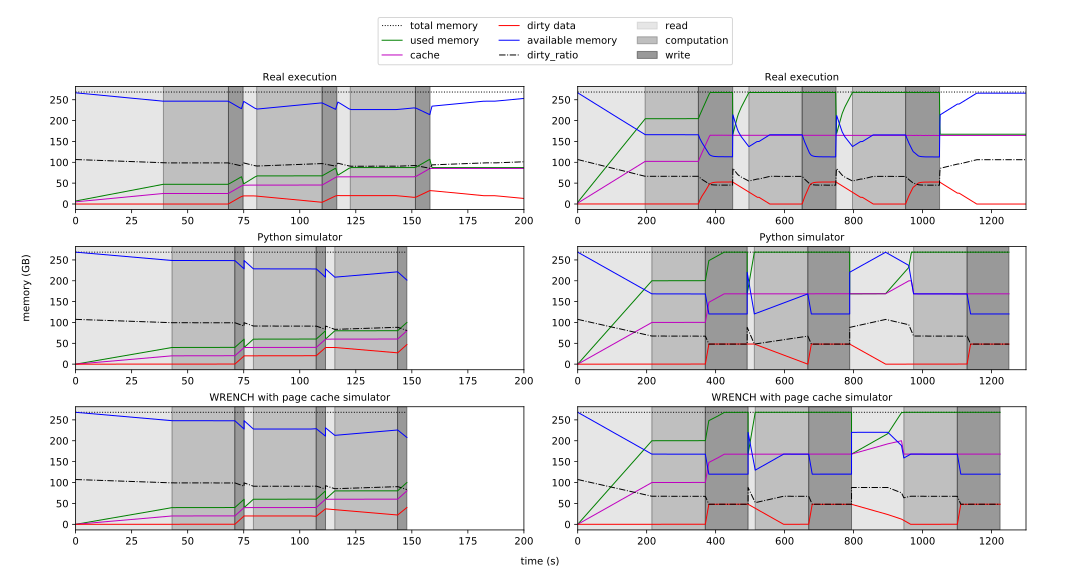
\includegraphics[width=\linewidth]{result/single/figures/single_memprof.pdf}
			\end{subfigure}
			\caption{Memory profiling results with different input file sizes}
			\label{fig:single_memprof}	
			\begin{subfigure}{\linewidth}
				\centering
   				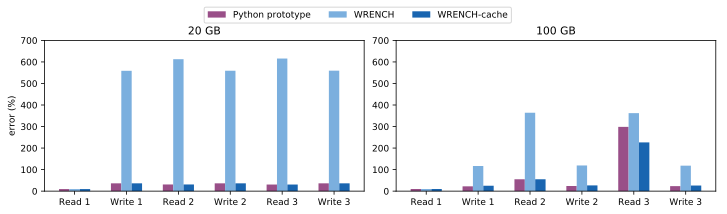
\includegraphics[width=\linewidth]{result/single/figures/single_errors.pdf}
			\end{subfigure}
			\caption{Simulation errors with different input file sizes}
			\label{fig:single_error}	
			\begin{subfigure}{\linewidth}
				\centering
   				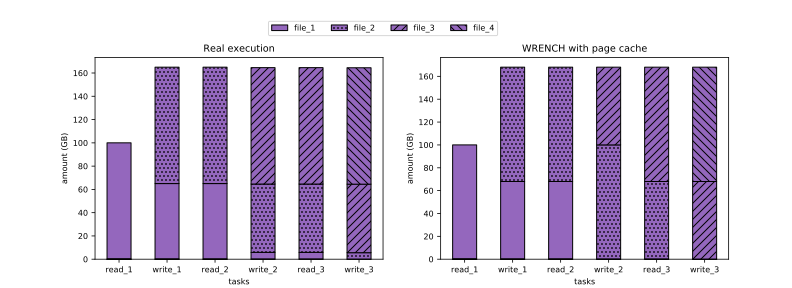
\includegraphics[width=\linewidth]{result/single/figures/cached_files.pdf}
			\end{subfigure}	
			\label{fig:single_cache}
   			\caption{Amount of file data in cache after each I/O activity with 100GB of input}
			\end{figure*}			

			This longer read can be explained with the amount of cached data of files 
			at the beginning of the read in reality and simulators shown in 
			Figure~\ref{fig:single_cache}. 			
			In this figure, \textit{file$<$i$>$} is the input of \textit{read$<$i$>$} and 
			output of \textit{write$<$i-1$>$}. 
			In the real execution, after \textit{write2}, which writes \textit{file3}, 
			all data of \textit{file3} is in cache (Figure~\ref{fig:fincore_real}). 
			Thus, in \textit{read3}, \textit{file3} is read with memory bandwidth. 
			But in our simulator, after \textit{write2}, only a part of \textit{file3} 
			remains in cache (Figure~\ref{fig:fincore_wrench}). 
			The reason is while \textit{file3}  is being written, the page cache is saturated, 
			eviction is then evoked to evict data from page cache, make space 
			available for \textit{file3}. 
			However, because the evicted amount is less than required, 
			some \textit{file3} data is evicted after being written, make \textit{file3} 
			partially cached. 
			As a result, in \textit{read3}, only a part of \textit{file3} is read from cache 
			with memory bandwidth, a part of it is read from disk with disk read bandwidth, 
			which is many times slower, leading to longer read time. 			
			
			In summary, in this single-threaded experiment, our model can accurately 
			simulate I/O time as well as the internal memory behavior. 
			This can help confirm that our model is on a right track and 
			it can be further improved to achieve higher accuracy.
			
		\subsection{Multi-threaded experiment}
		
			\begin{figure*}		
			\begin{subfigure}{\linewidth}
				\centering
   				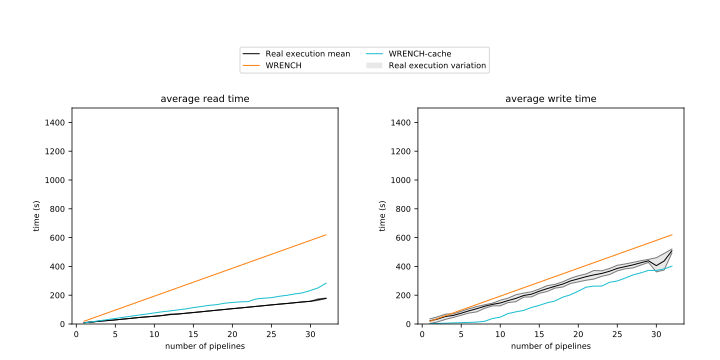
\includegraphics[width=\linewidth]{result/multi/figures/multi_local.pdf}
			\end{subfigure}		
			\caption{I/O time with different numbers of concurrent pipeline}
			\label{fig:multi_local}
			\end{figure*}		
			
			In this experiment, the results are analyzed in terms of average I/O time 
			of concurrent pipelines shown in Figure~\ref{fig:multi_local}.
			
			As is shown in the figure, when the number of pipelines increases, 
			the average read time raises accordingly because the amount of data 
			increases but memory and disk bandwidths are fixed and shared between pipelines. 
			In comparison with original WRENCH, the result from WRENCH with page cache are closer 
			to reality. 
			Especially, when it comes to the average write time, 
			although the trend in reality is more complex, our WRENCH with page cache 
			simulator can still capture the pattern in real execution.
			In both, the average write time gradually increases before surging with the 
			same slopes after the number of pipelines reaches 10. 
			This can be explained that with less than 10 concurrent pipelines, 
			the page cache is not saturated, so all files can be written entirely to 
			cache with memory bandwidth in a short time. 
			After the page cache is saturated with dirty data (at around 
			10 concurrent pipelines in this experiment), this dirty data needs 
			to be flushed in order to make space available for writing new data to cache. 
			This dirty data is flushed to disk with disk bandwidth, which is much  
			slower than memory bandwidth. 
			The more pipelines we have, the more data needs to be written, the more data 
			needs to be flushed, leading to a sharper increase in the average write time. 
			
			To conclude, the results from WRENCH with page cache simulator show that 
			our model can also simulate I/O with page cache accurately in a 
			multi-threaded application.  
			
		\subsection{Remote storage}
		
		\subsection{Real application}


	\section{Discussion and Future Work}
		\begin{itemize}
			\item Read order: disk, inactive list, then active list. 
			\item Cache eviction mechanism not evicting active list, leads to evicting file being written.
			\item Sensitivity of the simulator on the variation of memory and disk bandwidth. 
			\item Our model does not support random I/O and readahead.
			\item Disk state save/restore when hosts are turned on/off.
		\end{itemize}
	\section{CFI for cluster}
\bibliographystyle{plain}
\bibliography{citation}

\end{document}
